% ============================================================
%  Ocean Wave Theories — IEEE Two-Column Journal Format
% ============================================================
\documentclass[journal,10pt,twocolumn]{IEEEtran}

\usepackage{amsmath,amsfonts,amssymb,amsthm}
\usepackage{graphicx}
\usepackage{float}
\usepackage{booktabs}
\usepackage{array}
\usepackage{hyperref}
\usepackage{caption}
\usepackage{subcaption}
\usepackage{siunitx}
\usepackage{xcolor}
\usepackage{multirow}
\usepackage{cite}
\usepackage{tikz}
\usepackage{pgfplots}
\pgfplotsset{compat=1.18}

\newcolumntype{L}[1]{>{\raggedright\let\newline\\\arraybackslash\hspace{0pt}}m{#1}}
\newcolumntype{C}[1]{>{\centering\let\newline\\\arraybackslash\hspace{0pt}}m{#1}}
\newcolumntype{R}[1]{>{\raggedleft\let\newline\\\arraybackslash\hspace{0pt}}m{#1}}

% ============================================================
\begin{document}

\title{Ocean Wave Theories: From Classical Solutions to Modern Spectral Models}

\author{Various Generative AI\\Prompts by Mikhail Grushinskiy}

\maketitle

\begin{abstract}
The study of ocean waves represents a cornerstone of coastal and offshore engineering,
geophysics, and naval architecture, evolving over more than two centuries.
This review traces the historical development of wave theory from Gerstner's trochoidal
solution and Airy's foundational linear wave theory through Stokes' nonlinear corrections,
cnoidal and solitary-wave theory for shallow water, and Fenton's higher-order formulations.
The paper covers statistical and spectral representations essential for describing the
random nature of the sea, notably the Pierson--Moskowitz and JONSWAP spectra.
Governing Navier--Stokes equations and their simplifications are derived, and velocity
and acceleration fields for each major theory are compared.
A Le M\'ehaut\'e-style applicability diagram is included to summarize the regimes of
validity of the principal deterministic wave theories.
Industrial applications are discussed, including shallow- and deep-water wave regimes,
with practical tables for wave periods, lengths, and heights.
Finally, the specific models applied in contemporary offshore industries for different
design scenarios are summarized, including a brief modern note on rogue-wave mechanisms
and design relevance.
\end{abstract}

\begin{IEEEkeywords}
Ocean waves, Airy wave theory, Stokes waves, cnoidal wave theory,
solitary waves, JONSWAP spectrum, Pierson--Moskowitz spectrum,
Fenton stream function, rogue waves, Benjamin--Feir instability,
wave kinematics, offshore engineering.
\end{IEEEkeywords}

% ============================================================
\section{Introduction}
\label{sec:intro}

Ocean waves are a ubiquitous and powerful natural phenomenon, driven primarily by wind
transferring energy to the water surface.
Accurate prediction of wave kinematics (velocities, accelerations) and dynamics (forces,
energy) is critical for the design and operation of offshore structures (platforms, wind
turbines), ships, and coastal defenses.
The mathematical challenge of describing water waves is profound, involving nonlinear
boundary conditions at the free surface, making it one of the classic problems of fluid
dynamics.

The evolution of ocean wave theory is a journey from exact but restrictive solutions to
linearized approximations, then back to increasingly accurate nonlinear and statistical
descriptions.
Section~\ref{sec:history} details the historical context.
Section~\ref{sec:ns} establishes the governing equations.
Sections~\ref{sec:gerstner}--\ref{sec:fenton} dissect the key deterministic wave
theories, including their ranges of applicability.
Section~\ref{sec:spectral} introduces spectral models for irregular seas.
Section~\ref{sec:realwaves} discusses depth effects and practical parameter ranges.
Section~\ref{sec:industrial} summarizes industrial applications, and
Section~\ref{sec:conclusion} concludes.

% ============================================================
\section{Historical Development of Wave Theory}
\label{sec:history}

\subsection{Early Exact Solutions: The Gerstner Wave (1802)}
In 1802, Franz Joseph von Gerstner presented the first exact solution to the governing
equations for a wave propagating on the surface of an ideal fluid.
His \emph{trochoidal wave} described water particle motion as closed circular orbits,
larger at the surface and decaying with depth.
However, the flow field is rotational ($\nabla \times \mathbf{u} \neq 0$), whereas wind
waves are typically considered irrotational, limiting its use in fundamental fluid
dynamics.

\subsection{Linearization and the Foundation: Airy Theory (1841)}
Sir George Biddell Airy introduced a radical simplification in 1841: the small-amplitude
assumption $ak \ll 1$ (where $a$ is amplitude and $k$ is wavenumber).
This linearized the free-surface boundary conditions, yielding \emph{Airy wave theory}
(linear wave theory, LWT) and the vital dispersion relation
$\omega^2 = gk \tanh(kh)$.
Airy theory remains the fundamental building block for most engineering calculations.

\subsection{Nonlinear Developments: Stokes Theory (1847)}
Sir George Gabriel Stokes addressed steep-wave inaccuracies in 1847 by seeking a
solution as a perturbation series in wave steepness $\epsilon = ak$.
\emph{Stokes wave theory} added higher-order correction terms that produce crest--trough
asymmetry (sharp crests, flat troughs) and open particle orbits, enabling net mass
transport (\emph{Stokes drift}).

\subsection{Shallow-Water Nonlinear Theory: Cnoidal and Solitary Waves}
As the focus of engineering extended from deep-water swell to coastal and harbour
environments, it became clear that steepness alone is not the best measure of
nonlinearity in shallow water.
Long waves in finite depth are better described by cnoidal-wave solutions associated
with the Korteweg--de Vries framework, and by their solitary-wave limit for extreme
long-wave cases \cite{LeMehaute1976,Fenton1990,DNVC205}.

\subsection{Modern Higher-Order Expansions: Fenton's Theory (1980s)}
J.~D.~Fenton used computer algebra and Fourier-based formulations to derive highly
accurate nonlinear wave solutions, including stream-function approaches suitable for
steep waves and shallow-water transition regimes \cite{Fenton1990}.
These formulations underpin many modern offshore engineering tools.

\subsection{Spectral Approaches: Embracing Randomness (Mid-20th Century)}
Real ocean waves are irregular and random.
The sea surface is modeled as a superposition of infinite linear (Airy) components with
random phases; its statistics are described by the \emph{variance spectrum} $S(\omega)$.
\begin{itemize}
  \item \textbf{Pierson and Moskowitz (1964)} proposed an empirical spectrum for a
    \emph{fully developed sea} where energy input from wind balances dissipation.
  \item The \textbf{JONSWAP} project (1973) found that fetch-limited North Sea waves
    have a sharper spectral peak, leading to the JONSWAP spectrum now standard for
    offshore design.
\end{itemize}

% ============================================================
\section{Navier--Stokes Equations as Governing Framework}
\label{sec:ns}

All classical wave theories derive from the fundamental laws of fluid motion.
For an incompressible fluid the governing equations are:
\begin{enumerate}
  \item \textbf{Continuity:}
    \begin{equation}
      \nabla \cdot \mathbf{u} = 0
      \label{eq:continuity}
    \end{equation}
  \item \textbf{Momentum:}
    \begin{equation}
      \rho \!\left[\frac{\partial \mathbf{u}}{\partial t}
        + (\mathbf{u} \cdot \nabla)\mathbf{u}\right]
        = -\nabla p + \mu\nabla^2\mathbf{u} + \rho\mathbf{g}
      \label{eq:navierstokes}
    \end{equation}
\end{enumerate}
where $\mathbf{u}=(u,v,w)$ is velocity, $p$ pressure, $\rho$ density, $\mu$ dynamic
viscosity, and $\mathbf{g}=(0,0,-g)$.

\subsection{Simplifications for Ideal Flow}
Neglecting viscosity ($\mu=0$) and assuming irrotational flow
($\nabla\times\mathbf{u}=0$) allows the velocity to be written as
$\mathbf{u}=\nabla\phi$.
Substituting into~\eqref{eq:continuity} yields \textbf{Laplace's equation}:
\begin{equation}
  \nabla^2\phi = 0.
  \label{eq:laplace}
\end{equation}
The problem reduces to solving~\eqref{eq:laplace} subject to:
\begin{enumerate}
  \item \textbf{Kinematic bottom boundary condition (BBC)} at $z=-h$:
    \begin{equation}
      \frac{\partial\phi}{\partial z} = 0.
    \end{equation}
  \item \textbf{Kinematic free-surface boundary condition (FSBC)} at $z=\eta$:
    \begin{equation}
      \frac{\partial\eta}{\partial t}
        + \frac{\partial\phi}{\partial x}\frac{\partial\eta}{\partial x}
        + \frac{\partial\phi}{\partial y}\frac{\partial\eta}{\partial y}
        = \frac{\partial\phi}{\partial z}.
    \end{equation}
  \item \textbf{Dynamic FSBC} (constant pressure at the surface) via Bernoulli:
    \begin{equation}
      \frac{\partial\phi}{\partial t}
        + \frac{1}{2}|\nabla\phi|^2 + g\eta = 0
        \quad\text{at } z=\eta.
    \end{equation}
\end{enumerate}
The nonlinearity of these conditions, which must be applied at the unknown surface
$z=\eta(x,y,t)$, gives rise to the different wave theories.

% ============================================================
\section{Trochoidal (Gerstner) Waves}
\label{sec:gerstner}

\subsection{Formulation and Solution}
Gerstner defined the Lagrangian motion of each water particle.
For a wave propagating in the $x$-direction, the position of a particle with mean
position $(X,Z)$ is:
\begin{align}
  x &= X - \frac{a}{k}e^{kZ}\sin(kX-\omega t), \\
  z &= Z + \frac{a}{k}e^{kZ}\cos(kX-\omega t),
\end{align}
with dispersion relation $\omega^2 = gk$ (identical to deep-water linear waves).
Setting $Z=0$ gives the trochoidal free surface:
\begin{align}
  x_s &= X - \frac{a}{k}\sin(kX-\omega t), \\
  \eta &= \frac{a}{k}\cos(kX-\omega t),
\end{align}
which is sharper at the crest and flatter at the trough than a sinusoid.

\subsection{Velocity and Acceleration Fields}
\begin{align}
  u   &= a\omega e^{kZ}\cos(kX-\omega t), \\
  w   &= a\omega e^{kZ}\sin(kX-\omega t), \\
  a_x &= a\omega^2 e^{kZ}\sin(kX-\omega t), \\
  a_z &= -a\omega^2 e^{kZ}\cos(kX-\omega t).
\end{align}
Non-zero vorticity $\zeta = \partial u/\partial z - \partial w/\partial x$ confirms the
flow is rotational.

\subsection{Limitations and Applications}
The rotational nature violates the irrotationality assumption standard in wind-generated
wave analysis, and Gerstner waves cannot satisfy the zero-pressure condition for a
stratified fluid.
Although rarely used for engineering load calculations, the parametric simplicity of
the formulation has found application in computer graphics for generating realistic ocean
surfaces.

% ============================================================
\section{Airy (Linear) Wave Theory}
\label{sec:airy}

\subsection{Assumptions and Linearization}
Airy theory assumes inviscid, incompressible, irrotational flow; small wave steepness
$\epsilon=ak\ll1$; uniform depth $h$; and a plane wave (2D).
The small-steepness assumption linearizes the FSBCs by applying them at the mean water
level $z=0$ rather than at $z=\eta$.

\subsection{Velocity Potential and Surface Profile}
The solution to~\eqref{eq:laplace} with linearized boundary conditions is:
\begin{equation}
  \phi(x,z,t) = \frac{ag}{\omega}
    \frac{\cosh[k(z+h)]}{\cosh(kh)}\sin(kx-\omega t),
  \label{eq:airypotential}
\end{equation}
with surface elevation:
\begin{equation}
  \eta(x,t) = a\cos(kx-\omega t) = \frac{H}{2}\cos(kx-\omega t).
  \label{eq:airyeta}
\end{equation}

\subsection{Velocity and Acceleration Fields}
From $\mathbf{u}=\nabla\phi$:
\begin{align}
  u &= a\omega\frac{\cosh[k(z+h)]}{\sinh(kh)}\cos(kx-\omega t), \\
  w &= a\omega\frac{\sinh[k(z+h)]}{\sinh(kh)}\sin(kx-\omega t).
\end{align}
Eulerian accelerations:
\begin{align}
  a_x &= -a\omega^2\frac{\cosh[k(z+h)]}{\sinh(kh)}\sin(kx-\omega t), \\
  a_z &= -a\omega^2\frac{\sinh[k(z+h)]}{\sinh(kh)}\cos(kx-\omega t).
\end{align}

\subsection{Dispersion Relation}
\begin{equation}
  \omega^2 = gk\tanh(kh),
  \label{eq:dispersion}
\end{equation}
linking wave period $T=2\pi/\omega$, wavelength $\lambda=2\pi/k$, and depth $h$.
Wave celerity $c=\omega/k$ becomes:
\begin{equation}
  c = \sqrt{\frac{g\lambda}{2\pi}\tanh\!\left(\frac{2\pi h}{\lambda}\right)},
\end{equation}
showing that longer waves travel faster (\emph{dispersion}) and that waves slow in
shallow water (\emph{shoaling}).

\subsection{Pressure Field}
The linearized Bernoulli equation gives:
\begin{equation}
  p = -\rho gz + \rho g\eta\,K_p(z),
  \label{eq:airypressure}
\end{equation}
where $K_p(z)=\cosh[k(z+h)]/\cosh(kh)$ is the pressure response factor.
The first term is hydrostatic; the second is the dynamic wave-induced pressure,
decaying with depth.

\subsection{Industrial Use and Limitations}
Airy theory is the workhorse of ocean engineering:
it underpins spectral analysis (Section~\ref{sec:spectral}), the Morison equation for
loads on slender members, and operational wave forecasting models (WAM, WAVEWATCH~III).
Its primary limitation is inaccuracy for steep waves, where it fails to predict
asymmetry, higher harmonics, and mass transport.

% ============================================================
\section{Stokes Wave Theory}
\label{sec:stokes}

\subsection{Perturbation Approach}
Stokes sought a solution as a power series in $\epsilon=ak$:
\begin{align}
  \phi &= \epsilon\phi_1 + \epsilon^2\phi_2 + \epsilon^3\phi_3 + \cdots, \\
  \eta &= \epsilon\eta_1 + \epsilon^2\eta_2 + \epsilon^3\eta_3 + \cdots,
\end{align}
solved order-by-order, with $\phi_1$ and $\eta_1$ being the linear (Airy) solutions.

\subsection{Second-Order Theory}
With $\theta=kx-\omega t$, the second-order surface elevation is:
\begin{equation}
  \eta = a\cos\theta
    + \frac{a^2k}{4}\frac{\cosh(kh)(2+\cosh(2kh))}{\sinh^3(kh)}\cos 2\theta.
\end{equation}
In \textbf{deep water} this simplifies to:
\begin{align}
  \eta &= a\cos\theta + \tfrac{1}{2}a^2k\cos 2\theta, \\
  \phi &= \frac{ag}{\omega}e^{kz}\sin\theta
         + \frac{3}{8}a^2\omega e^{2kz}\sin 2\theta.
\end{align}
The second-order correction is positive at the crest and negative at the trough,
producing the characteristic \emph{crest--trough asymmetry}.

\subsection{Higher-Order Properties}
Key nonlinear features include:
\begin{itemize}
  \item \textbf{Phase speed increase:} Wave speed depends on wave height.
  \item \textbf{Stokes drift:} Open particle orbits produce net mass transport in the
    direction of propagation.
  \item \textbf{Asymmetric kinematics:} Horizontal velocity under the crest exceeds
    that under the trough.
\end{itemize}
Stokes 2nd and 5th order theories are codified in design standards for intermediate to
deep water calculations \cite{DNVC205}.

% ============================================================
\section{Wave-Theory Applicability and Shallow-Water Nonlinearity}
\label{sec:applicability}

\subsection{Quantified applicability diagram}
The classical Le M\'ehaut\'e chart is best understood today through the quantified update
of Zhao, Wang, and Liu, who redrew the selection map in the
\((h/L,\;H/L)\) plane, where \(h/L\) measures frequency dispersion and \(H/L\) measures
nonlinearity.
That choice is tighter and less arbitrary than the older textbook redraws in
\((h/gT^2,\;H/gT^2)\), while remaining directly interpretable for engineering wave
selection.
The breaking limit is represented by Miche/Fenton-type steepness, the division between
Stokes and cnoidal regimes is governed by the Ursell number, and the cnoidal subregions
are further split by the elliptic parameter \(m\).

\begin{figure*}[t]
\centering
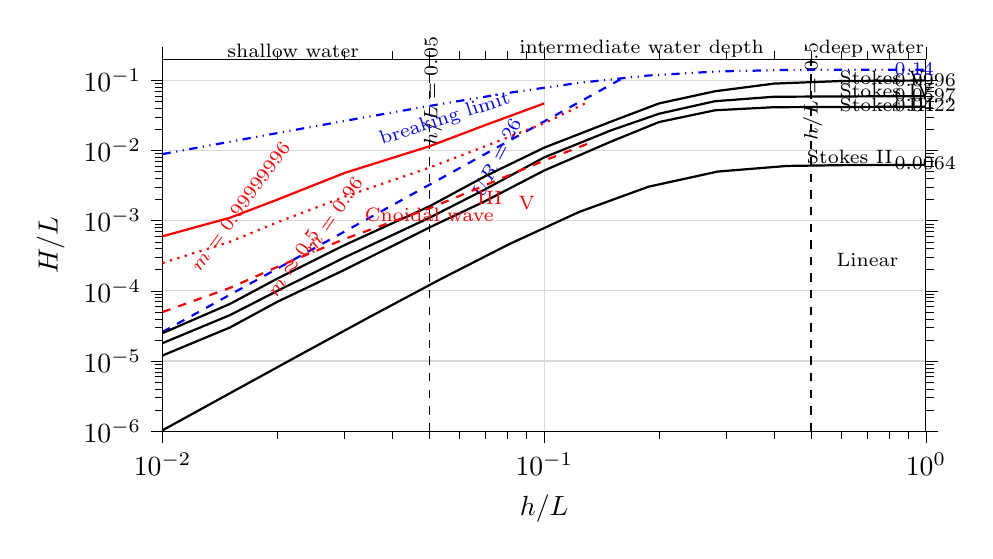
\begin{tikzpicture}
\begin{loglogaxis}[
  width=0.93\textwidth,
  height=0.52\textwidth,
  xmin=1e-2, xmax=1,
  ymin=1e-6, ymax=2e-1,
  xlabel={$h/L$},
  ylabel={$H/L$},
  xtick={1e-2,1e-1,1e0},
  ytick={1e-6,1e-5,1e-4,1e-3,1e-2,1e-1},
  grid=major,
  major grid style={draw=black!15},
  tick align=outside,
  tick style={black},
  axis line style={black},
  legend style={draw=none, fill=none, font=\scriptsize},
  clip=false
]

% depth-regime separators
\addplot[black, dashed] coordinates {(0.05,1e-6) (0.05,2e-1)};
\addplot[black, dashed] coordinates {(0.5,1e-6) (0.5,2e-1)};

\node[font=\scriptsize, anchor=south] at (axis cs:0.022,1.55e-1) {shallow water};
\node[font=\scriptsize, anchor=south] at (axis cs:0.18,1.55e-1) {intermediate water depth};
\node[font=\scriptsize, anchor=south] at (axis cs:0.72,1.55e-1) {deep water};

\node[font=\scriptsize, rotate=90] at (axis cs:0.051,7e-2) {$h/L=0.05$};
\node[font=\scriptsize, rotate=90] at (axis cs:0.505,7e-2) {$h/L=0.5$};

% exact UR=26 line in h/L, H/L variables: UR=(H/L)/(h/L)^3
\addplot[blue, dashed, thick] coordinates {
  (0.01000,2.6e-05)
  (0.01359,6.5309e-05)
  (0.01848,0.000164049)
  (0.02512,0.000412072)
  (0.03415,0.00103508)
  (0.04642,0.0026)
  (0.06310,0.0065309)
  (0.08577,0.0164049)
  (0.11659,0.0412072)
  (0.15849,0.103508)
};
\node[font=\scriptsize, text=blue, rotate=63] at (axis cs:0.075,0.008) {$UR=26$};

% exact Miche/Fenton-type breaking limit: H/L = 0.142 tanh(2 pi h/L)
\addplot[blue, dash dot dot, thick] coordinates {
  (0.01000,0.0089104)
  (0.01520,0.0135198)
  (0.02310,0.0204677)
  (0.03511,0.0308287)
  (0.05337,0.0459069)
  (0.08111,0.0666933)
  (0.12328,0.0922444)
  (0.18738,0.117379)
  (0.28480,0.13429)
  (0.43288,0.140773)
  (0.65793,0.141927)
  (1.00000,0.141999)
};
\node[font=\scriptsize, text=blue, rotate=18] at (axis cs:0.055,0.028) {breaking limit};

% linear / Stokes-II boundary
\addplot[black, thick] coordinates {
  (0.01000,1.03083e-06)
  (0.01520,3.60699e-06)
  (0.02310,1.25646e-05)
  (0.03511,4.3318e-05)
  (0.05337,0.000145867)
  (0.08111,0.00046595)
  (0.12328,0.00132917)
  (0.18738,0.00304754)
  (0.28480,0.00502103)
  (0.43288,0.00603736)
  (0.65793,0.00623718)
  (1.00000,0.00624983)
};
\node[font=\scriptsize, anchor=west] at (axis cs:0.55,2.8e-4) {Linear};
\node[font=\scriptsize, anchor=west] at (axis cs:0.78,0.0066) {0.0064};

% tighter digitized redraw of Zhao 2024 higher-order Stokes boundaries
\addplot[black, thick] coordinates {
  (0.010,1.2e-05)
  (0.015,3.0e-05)
  (0.020,7.0e-05)
  (0.030,2.0e-04)
  (0.050,8.0e-04)
  (0.070,1.9e-03)
  (0.100,5.2e-03)
  (0.150,1.35e-02)
  (0.200,2.55e-02)
  (0.280,3.75e-02)
  (0.400,4.15e-02)
  (1.000,4.22e-02)
};
\node[font=\scriptsize, anchor=west] at (axis cs:0.46,0.0082) {Stokes II};
\node[font=\scriptsize, anchor=west] at (axis cs:0.78,0.0435) {0.0422};

\addplot[black, thick] coordinates {
  (0.010,1.8e-05)
  (0.015,4.5e-05)
  (0.020,1.0e-04)
  (0.030,3.0e-04)
  (0.050,1.1e-03)
  (0.070,2.8e-03)
  (0.100,8.0e-03)
  (0.150,1.95e-02)
  (0.200,3.35e-02)
  (0.280,5.05e-02)
  (0.400,5.85e-02)
  (1.000,5.97e-02)
};
\node[font=\scriptsize, anchor=west] at (axis cs:0.56,0.045) {Stokes III};
\node[font=\scriptsize, anchor=west] at (axis cs:0.78,0.0615) {0.0597};

\addplot[black, thick] coordinates {
  (0.010,2.5e-05)
  (0.015,6.5e-05)
  (0.020,1.5e-04)
  (0.030,4.5e-04)
  (0.050,1.6e-03)
  (0.070,4.3e-03)
  (0.100,1.1e-02)
  (0.150,2.6e-02)
  (0.200,4.7e-02)
  (0.280,7.0e-02)
  (0.400,9.0e-02)
  (0.600,9.8e-02)
  (1.000,9.96e-02)
};
\node[font=\scriptsize, anchor=west] at (axis cs:0.56,0.072) {Stokes IV};
\node[font=\scriptsize, anchor=west] at (axis cs:0.78,0.102) {0.0996};

% cnoidal boundaries digitized from the updated Zhao-style figure
\addplot[red, dashed, thick] coordinates {
  (0.010,5.0e-05)
  (0.015,1.1e-04)
  (0.020,2.2e-04)
  (0.030,5.5e-04)
  (0.050,1.5e-03)
  (0.070,3.2e-03)
  (0.100,7.2e-03)
  (0.130,1.25e-02)
};
\node[font=\scriptsize, text=red, rotate=56] at (axis cs:0.022,2.5e-04) {$m\approx0.5$};

\addplot[red, dotted, thick] coordinates {
  (0.010,2.5e-04)
  (0.015,5.0e-04)
  (0.020,9.5e-04)
  (0.030,2.2e-03)
  (0.050,5.7e-03)
  (0.070,1.15e-02)
  (0.100,2.45e-02)
  (0.130,4.9e-02)
};
\node[font=\scriptsize, text=red, rotate=55] at (axis cs:0.028,0.0012) {$m=0.96$};

\addplot[red, solid, thick] coordinates {
  (0.010,6.0e-04)
  (0.015,1.1e-03)
  (0.020,2.0e-03)
  (0.030,4.8e-03)
  (0.050,1.15e-02)
  (0.070,2.3e-02)
  (0.100,4.7e-02)
};
\node[font=\scriptsize, text=red, rotate=54] at (axis cs:0.016,0.0016) {$m=0.99999996$};

\node[font=\scriptsize, text=red] at (axis cs:0.050,0.0012) {Cnoidal wave};
\node[font=\scriptsize, text=red] at (axis cs:0.072,0.0021) {III};
\node[font=\scriptsize, text=red] at (axis cs:0.090,0.0018) {V};

\node[font=\scriptsize, anchor=west] at (axis cs:0.56,0.108) {Stokes V};
\node[font=\scriptsize, anchor=west, text=blue] at (axis cs:0.78,0.142) {0.14};

\end{loglogaxis}
\end{tikzpicture}
\caption{Quantified Le M\'ehaut\'e-style applicability diagram redrawn in the
\((h/L,\;H/L)\) plane, following the 2024 Zhao--Wang--Liu update rather than the older
qualitative textbook sketch.
The \(UR=26\) divider and the breaking curve are plotted from the published update,
while the cnoidal-order and solitary-wave boundaries are a tight vector redraw of the
authors' updated figure.}
\label{fig:lemehaute}
\end{figure*}

\subsection{Cnoidal wave theory}
For shallow water, the relevant nonlinearity is better measured by the
\emph{Ursell number},
\begin{equation}
  UR=\frac{HL^2}{h^3}
  =\frac{H/L}{(h/L)^3}.
\end{equation}
Large values of \(UR\) indicate that nonlinearity dominates frequency dispersion, in
which case Stokes expansions cease to be the natural asymptotic description and
cnoidal-wave theory becomes more appropriate.
This is precisely the transition that the quantified applicability chart seeks to mark.

A periodic cnoidal wave may be written in terms of the Jacobi elliptic cosine as
\begin{equation}
  \eta(x,t)=\eta_2+H\,\mathrm{cn}^2\!\left(
  \frac{2K(m)}{L}(x-ct),\,m\right),
\end{equation}
where \(K(m)\) is the complete elliptic integral of the first kind and \(m\in(0,1)\) is
the elliptic modulus.
Compared with Stokes waves, cnoidal waves have sharper crests and flatter, broader
troughs.
As \(m\to1\), the wavelength tends to infinity and the cnoidal solution approaches the
solitary-wave limit.

% ============================================================
\section{Fenton's Higher-Order Theory}
\label{sec:fenton}

\subsection{Stream Function Method}
Working in a reference frame moving with wave celerity $c$, the flow becomes steady.
The stream function $\psi$ satisfies:
\begin{align}
  u - c &= -\frac{\partial\psi}{\partial z}, \quad
  w      = \frac{\partial\psi}{\partial x},
\end{align}
and is expanded as a Fourier series:
\begin{equation}
  \psi(x,z) = -cz + \sum_{n=1}^{N} B_n \sin[nk(x-ct)]
    \frac{\cosh[nk(z+h)]}{\cosh(nkh)},
\end{equation}
where coefficients $B_n$ and celerity $c$ are found numerically by minimizing the
error in the dynamic FSBC over $N$ collocation points on the free surface.

\subsection{Advantages and Application}
This formulation converges faster than the Stokes perturbation series for very steep
waves.
Fenton's 5th- or 10th-order stream function theory is implemented in industry-standard
software and is considered accurate even for waves near the breaking limit
\cite{Fenton1990,DNVC205}.

% ============================================================
\section{Spectral Representations of Irregular Waves}
\label{sec:spectral}

\subsection{The Random Sea Concept}
A real sea state is modeled as a stationary Gaussian random process:
\begin{equation}
  \eta(t) = \sum_{i=1}^{N} a_i\cos(\omega_i t + \epsilon_i),
\end{equation}
where $\epsilon_i$ are random phases uniformly distributed on $[0,2\pi]$.

\subsection{The Variance Spectrum}
The wave variance spectrum $S_\eta(\omega)$ encodes how energy is distributed across
frequencies.
Significant wave height $H_s$ is related to the zeroth spectral moment:
\begin{equation}
  H_s \approx H_{m0} = 4\sqrt{m_0}, \quad
  m_0 = \int_0^\infty S_\eta(\omega)\,d\omega.
\end{equation}

\subsection{Pierson--Moskowitz Spectrum (1964)}
For a fully developed sea, the PM spectrum is:
\begin{equation}
  S_\eta(\omega) = \alpha g^2\omega^{-5}
    \exp\!\left[-\beta\!\left(\frac{\omega_p}{\omega}\right)^{\!4}\right],
\end{equation}
with $\alpha=8.1\times10^{-3}$, $\beta=0.74$, and peak frequency
$\omega_p = 0.855\,g/U_{19.5}$.
Rewritten in terms of $H_s$:
\begin{equation}
  S_\eta(\omega) = \frac{5}{16}H_s^2\omega_p^4\omega^{-5}
    \exp\!\left[-\frac{5}{4}\!\left(\frac{\omega_p}{\omega}\right)^{\!4}\right].
\end{equation}

\subsection{JONSWAP Spectrum (1973)}
For fetch-limited conditions the JONSWAP spectrum modifies the PM form:
\begin{equation}
  S_{\text{JS}}(\omega) = S_{\text{PM}}(\omega)\cdot
    \gamma^{\exp\!\left[-\frac{(\omega-\omega_p)^2}{2\sigma^2\omega_p^2}\right]},
\end{equation}
where $\gamma$ is the peak enhancement factor (typically 3.3; range 1--7), and
$\sigma=0.07$ for $\omega\le\omega_p$, $\sigma=0.09$ for $\omega>\omega_p$.
JONSWAP is the de facto standard for offshore structure design worldwide.

\subsection{Directional Spreading}
Real seas are multi-directional, modeled by:
\begin{equation}
  S(\omega,\theta) = S(\omega)\,D(\theta,\omega),
\end{equation}
where $D(\theta)\propto\cos^s(\theta)$ is a spreading function centered on the main
wave direction.

\subsection{Rogue and Freak Waves}
A modern review of ocean-wave theory should also acknowledge \emph{rogue} or
\emph{freak} waves: unusually large individual waves embedded in an otherwise random sea.
Operational offshore guidance commonly characterizes such events by criteria such as
\begin{equation}
  \frac{H_{\max}}{H_s} > 2
  \qquad \text{or} \qquad
  \frac{C_{\max}}{H_s} > 1.3,
\end{equation}
where $H_{\max}$ is the maximum individual wave height in a record and $C_{\max}$ is the
maximum crest elevation \cite{DNVC205}.

One important nonlinear mechanism is the Benjamin--Feir (modulational) instability of a
narrowband, steep wave train \cite{BenjaminFeir1967}.
Its strength is often summarized by the Benjamin--Feir index (BFI),
\begin{equation}
  \mathrm{BFI} = \sqrt{2}\,\frac{\varepsilon}{\nu},
\end{equation}
where $\varepsilon$ is spectral steepness and $\nu$ is spectral bandwidth.
Large BFI indicates enhanced susceptibility to nonlinear focusing, especially in
long-crested deep-water conditions.
However, field evidence suggests that rogue-wave occurrence in the real ocean is not
explained by BFI alone; directional spreading, crossing seas, current gradients, and
linear/dispersive focusing may all contribute \cite{Gemmrich2022,Hafner2021}.

The best-known measured example is the \emph{Draupner wave}, recorded on
1 January 1995 at the Draupner platform in the North Sea.
Its measurement transformed rogue waves from anecdotal reports into a concrete offshore
design concern \cite{ECMWFDraupner,DNVC205}.

% ============================================================
\section{Real Ocean Waves: Properties and Depth Effects}
\label{sec:realwaves}

\subsection{Practical Ranges of Wave Parameters}
Table~\ref{tab:waveparams} summarizes typical ranges for ocean wind waves.

\begin{table}[H]
  \centering
  \caption{Typical Ranges for Ocean Wind Waves}
  \label{tab:waveparams}
  \small
  \begin{tabular}{@{}lL{2.1cm}L{2.2cm}@{}}
    \toprule
    Parameter & Typical Range & Extreme Events \\
    \midrule
    Height $H$        & 0.5--6\,m
      & $>$30\,m estimated (N.~Atlantic); 19\,m recorded (North Sea) \\
    Period $T$        & 4--12\,s
      & 20--25\,s (distant storm swell) \\
    Length $\lambda$  & 25--225\,m
      & $\sim$800\,m ($T=25$\,s, deep water) \\
    Steepness $H/\lambda$ & 0.01--0.06
      & $\approx0.14$ (deep-water breaking limit) \\
    \bottomrule
  \end{tabular}
\end{table}

\subsection{Depth Classification and Effects}
The ratio $h/\lambda$ governs wave behavior.
Table~\ref{tab:depthtable} summarizes the three regimes.

\begin{table}[H]
  \centering
  \caption{Wave Classification by Relative Depth}
  \label{tab:depthtable}
  \small
  \begin{tabular}{@{}lL{1.4cm}L{1.4cm}L{1.6cm}@{}}
    \toprule
    Regime & Condition & Celerity $c$ & Particle Motion \\
    \midrule
    Deep
      & $h/\lambda>\tfrac{1}{2}$
      & $gT/(2\pi)$
      & Circular, decaying with depth \\
    Inter\-mediate
      & $\tfrac{1}{20}<h/\lambda<\tfrac{1}{2}$
      & Full dispersion relation
      & Elliptical, reaching bottom \\
    Shallow
      & $h/\lambda<\tfrac{1}{20}$
      & $\sqrt{gh}$
      & Nearly horizontal \\
    \bottomrule
  \end{tabular}
\end{table}

\begin{itemize}
  \item \textbf{Shoaling:} Speed and wavelength decrease; height increases to conserve
    energy as waves enter shallow water.
  \item \textbf{Refraction:} Waves bend toward depth contours due to celerity gradients
    across the wave front.
  \item \textbf{Breaking:} Waves break when steepness exceeds a threshold (spilling on
    gentle slopes; plunging on steep slopes).
\end{itemize}

The shallow-water regime is also the regime in which cnoidal and solitary-wave ideas
become practically important.
In dimensionless terms, depth alone is not sufficient to select the correct theory:
nonlinearity and dispersion must be considered jointly, which is precisely what the
Le M\'ehaut\'e chart in Fig.~\ref{fig:lemehaute} summarizes \cite{LeMehaute1976,Zhao2024}.

% ============================================================
\section{Industrial Usage Summary}
\label{sec:industrial}

Table~\ref{tab:industrial} summarizes recommended wave models for common offshore
engineering tasks.

\begin{table*}[t]
  \centering
  \caption{Application of Wave Models in Offshore Engineering}
  \label{tab:industrial}
  \small
  \begin{tabular}{@{}L{2.8cm}L{6.5cm}L{3.5cm}@{}}
    \toprule
    Design Aspect & Primary Wave Model & Rationale \\
    \midrule
    Fatigue analysis
      & Linear spectral model (Airy)
      & Computationally efficient; valid for small waves dominating fatigue
        accumulation; supports superposition of many sea states. \\[4pt]
    Global extreme loads (ship hull, platform)
      & JONSWAP spectrum $+$ 2nd/3rd-order Stokes kinematics
      & Captures statistical likelihood of extremes (spectrum) and enhanced crest
        kinematics (nonlinear theory). \\[4pt]
    Local loads (slamming, green water)
      & Fenton high-order or CFD
      & Requires highly accurate wave profile and kinematics at the extreme crest. \\[4pt]
    Shallow-water wave loading
      & Cnoidal (large $UR$), or stream function/Fourier near transition and near breaking
      & Stokes theory loses validity in very shallow water; cnoidal theory captures long,
        nonlinear shallow-water waves, while stream-function methods are preferred close
        to the transition region and near the limiting steep-wave boundary. \\[4pt]
    Wave forecasting
      & Linear spectral models (WAM, WAVEWATCH~III)
      & Global/regional spectral energy balance; linear physics dominates at large
        scale. \\
    \bottomrule
  \end{tabular}
\end{table*}

% ============================================================
\section{Chronology of Key Wave Models}
\label{sec:modeltable}

Table~\ref{tab:chronology} provides a chronological summary of the key ocean wave
models discussed in this paper.

\begin{table*}[t]
  \centering
  \caption{Chronology and Summary of Key Ocean Wave Models}
  \label{tab:chronology}
  \small
  \begin{tabular}{@{}L{2.3cm}lL{8.5cm}@{}}
    \toprule
    Model & Year & Key Characteristics and Applications \\
    \midrule
    Gerstner        & 1802
      & First exact solution. Rotational flow, trochoidal profile.
        Largely of historical/theoretical interest; used in computer graphics. \\
    Airy (Linear)   & 1841
      & Foundation of modern analysis. Irrotational, sinusoidal profile,
        dispersion relation. Used in spectral models, fatigue, and preliminary design. \\
    Stokes (2nd--5th) & 1847/modern
      & Perturbation series in wave steepness. Irrotational, asymmetric profile,
        mass transport. Standard for nonlinear extreme load calculations. \\
    Cnoidal / solitary & 1895/modern
      & Shallow-water nonlinear theory associated with long waves and large Ursell number.
        Used in coastal and harbour engineering; the solitary wave is recovered in the
        long-wave limit. \\
    Fenton (high-order) & 1980s
      & Numerical/stream-function solution. Highly accurate for steep waves near
        breaking and useful across transition regimes. Used for detailed crest
        kinematics in advanced structural analysis. \\
    Pierson--Moskowitz & 1964
      & Energy spectrum for fully developed seas. Base spectrum for many
        applications. \\
    JONSWAP         & 1973
      & Spectrum for fetch-limited seas (e.g., North Sea). Sharper spectral peak.
        Industry standard for extreme event design worldwide. \\
    Rogue-wave design guidance & modern
      & Statistical and nonlinear interpretation of extreme individual waves,
        including freak-wave criteria used in offshore design recommendations. \\
    \bottomrule
  \end{tabular}
\end{table*}

% ============================================================
\section{Conclusion}
\label{sec:conclusion}

The mathematical description of ocean waves has undergone a remarkable evolution driven
by the needs of science and engineering.
From Gerstner's elegant but restrictive trochoidal solution, the field advanced with
Airy's revolutionary linearization, providing the indispensable dispersion relation and
the framework for spectral analysis.
Stokes' nonlinear perturbation method explained wave asymmetry, a crucial step validated
by observation.
For shallow water, cnoidal and solitary-wave theories provided the correct nonlinear
long-wave description where steepness-based Stokes expansions cease to be appropriate.
The modern era, championed by Fenton and related numerical formulations, leverages
computational power to achieve high-fidelity solutions for the most extreme waves.

Today's engineering practice is a hybrid: the randomness of the sea is captured through
linear spectral models (Pierson--Moskowitz, JONSWAP), while the critical nonlinear
physics of extreme waves is incorporated via Stokes, cnoidal, or stream-function/Fenton
theories for load calculations.
This combination enables the safe and efficient design of structures that operate in the
dynamic and challenging ocean environment.
Modern offshore guidance additionally recognizes rogue or freak waves as a practical
design consideration, linking classical wave theory to contemporary reliability-based
assessment \cite{DNVC205}.

% ============================================================
\begin{thebibliography}{99}

\bibitem{LeMehaute1976}
B.~Le M\'ehaut\'e,
\emph{An Introduction to Hydrodynamics and Water Waves}.
New York, NY, USA: Springer, 1976.

\bibitem{Zhao2024}
K.~Zhao, Y.~Wang, and P.~L.-F.~Liu,
``A guide for selecting periodic water wave theories---Le M\'ehaut\'e (1976)'s graph revisited,''
\emph{Coastal Engineering}, vol.~188, Art.~104432, 2024.

\bibitem{Fenton1990}
J.~D.~Fenton,
``Nonlinear wave theories,''
in \emph{The Sea, Vol.~9: Ocean Engineering Science},
B.~Le M\'ehaut\'e and D.~M.~Hanes, Eds.
New York, NY, USA: Wiley, 1990, pp.~3--25.

\bibitem{DNVC205}
DNV GL,
\emph{DNVGL-RP-C205: Environmental Conditions and Environmental Loads},
Recommended Practice, Aug.~2017.

\bibitem{BenjaminFeir1967}
T.~B.~Benjamin and J.~E.~Feir,
``The disintegration of wave trains on deep water. Part 1. Theory,''
\emph{Journal of Fluid Mechanics}, vol.~27, no.~3, pp.~417--430, 1967.

\bibitem{Gemmrich2022}
J.~Gemmrich, T.~Breivik, A.~Kromer, L.~Lenain, and M.~A.~Donelan,
``Generation mechanism and prediction of an observed rogue wave,''
\emph{Scientific Reports}, vol.~12, Art.~1718, 2022.

\bibitem{Hafner2021}
D.~Hafner, C.~Gemmrich, and J.~M.~Janssen,
``Real-world rogue wave probabilities,''
\emph{Scientific Reports}, vol.~11, Art.~10084, 2021.

\bibitem{ECMWFDraupner}
ECMWF,
``What conditions led to the Draupner freak wave?''
\emph{ECMWF Newsletter}, no.~148, pp.~12--16, 2016.

\end{thebibliography}

% ============================================================
\end{document}
